\section{Medicion en continua}
\begin{frame}
	\frametitle{Mediciones en continua: Microfono}
	\begin{columns}[t]
		\column{0.6\textwidth}
		\begin{figure}[H]
			\centering
			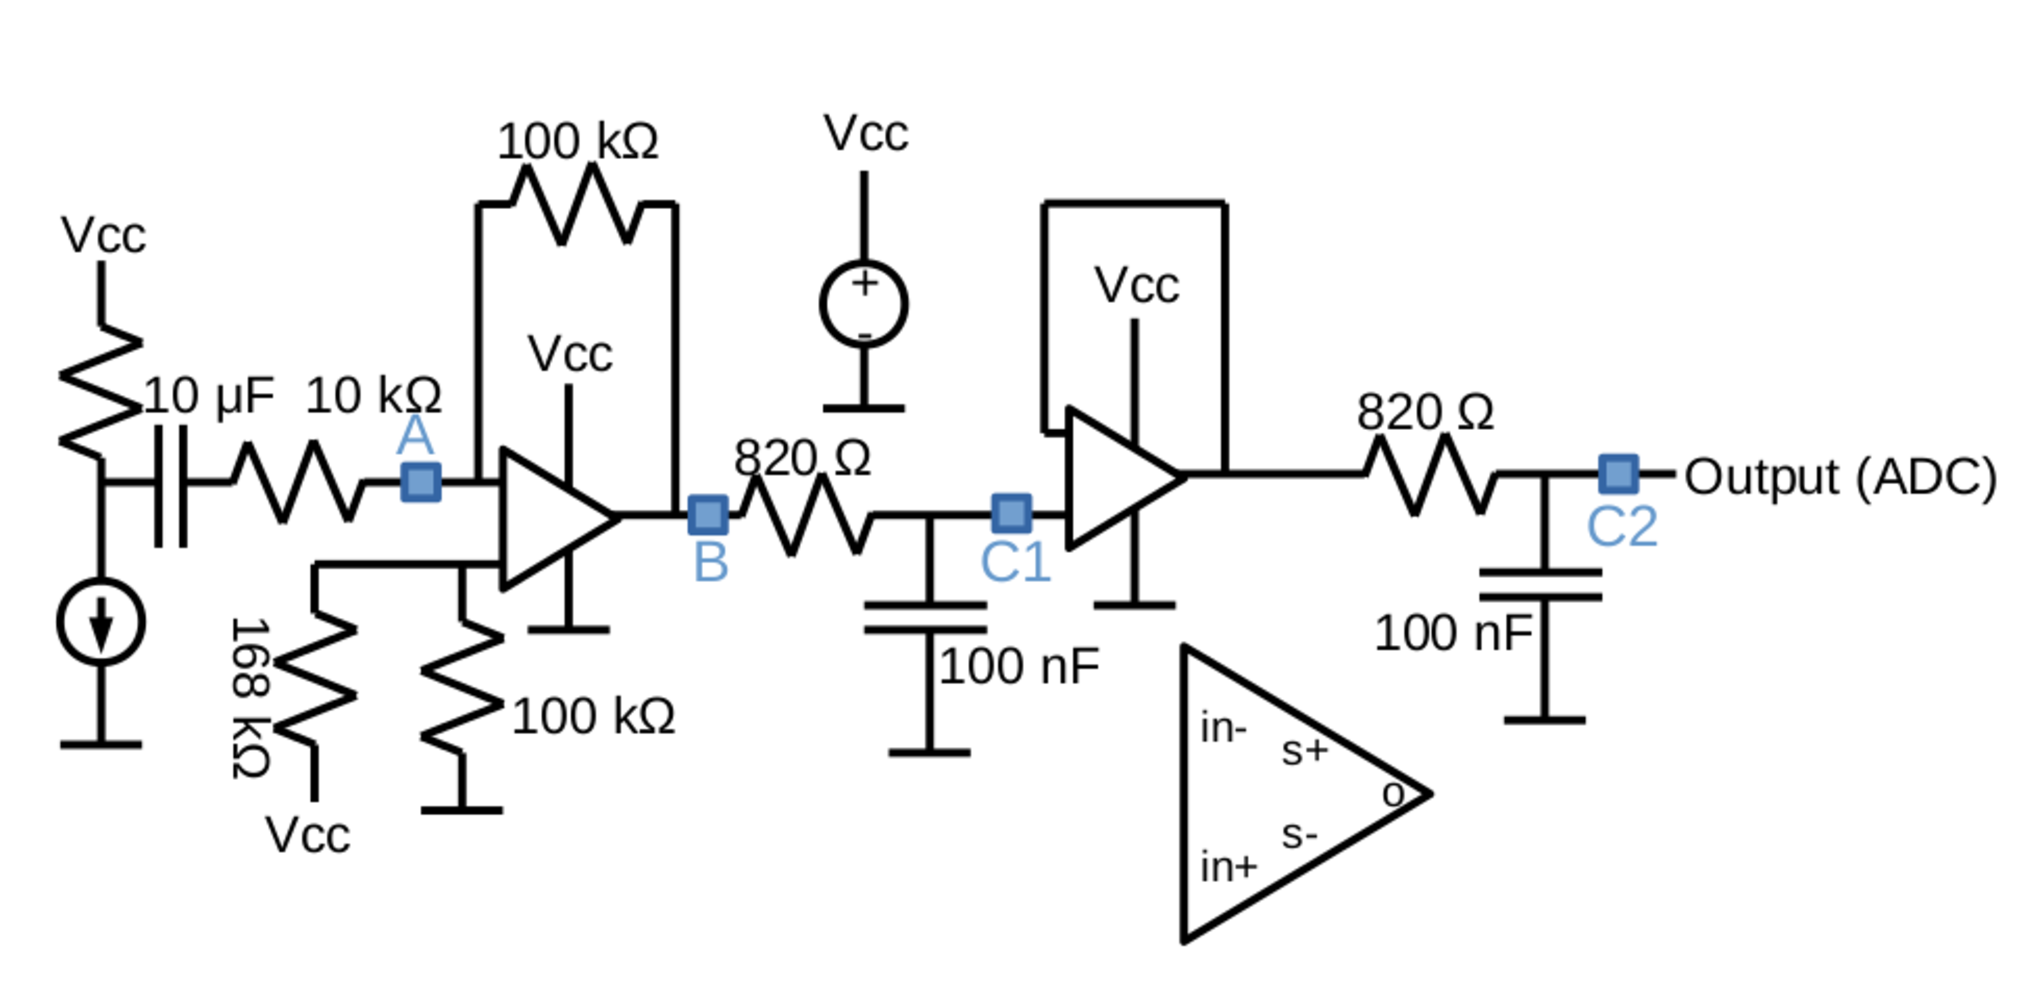
\includegraphics[scale=0.3]{AmpMic}	
		\end{figure}
		\column{0.4\textwidth}
		\begin{table}
			\centering
			\begin{tabular}{c|c}
				Punto & Tensión\\
				\hline \hline
				A & $(1.86;0.02)V$  \\
				\hline
				B & $(1.88;0.02)V$\\
				\hline
				C1 & $(1.87;0.02)V$\\
				\hline
				C2 & $(1.88;0.02)V$\\
				\hline
			\end{tabular}
		\end{table}
	\end{columns}
\end{frame}

\begin{frame}
\frametitle{Mediciones en continua: Microcontrolador}
	\begin{columns}[t]
		\column{0.6\textwidth}
		\begin{figure}
			\centering
			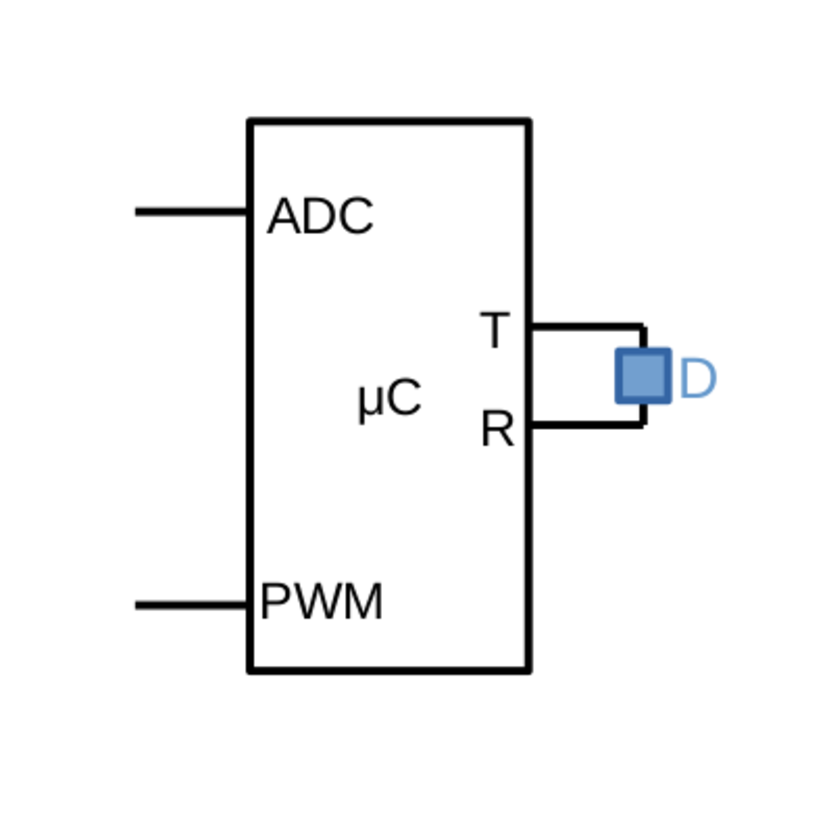
\includegraphics[scale=0.4]{MicroCon}	
		\end{figure}
		\column{0.4\textwidth}
		\begin{table}
			\centering
			\begin{tabular}{c|c}
				Punto & Tensión\\
				\hline \hline
				D & $(1.87;0.02)V$  \\
				\hline
			\end{tabular}
		\end{table}
	\end{columns}
\end{frame}

\begin{frame}
\frametitle{Mediciones en continua: Parlante}
	\begin{columns}[t]
		\column{0.6\textwidth}
		\begin{figure}
			\centering
			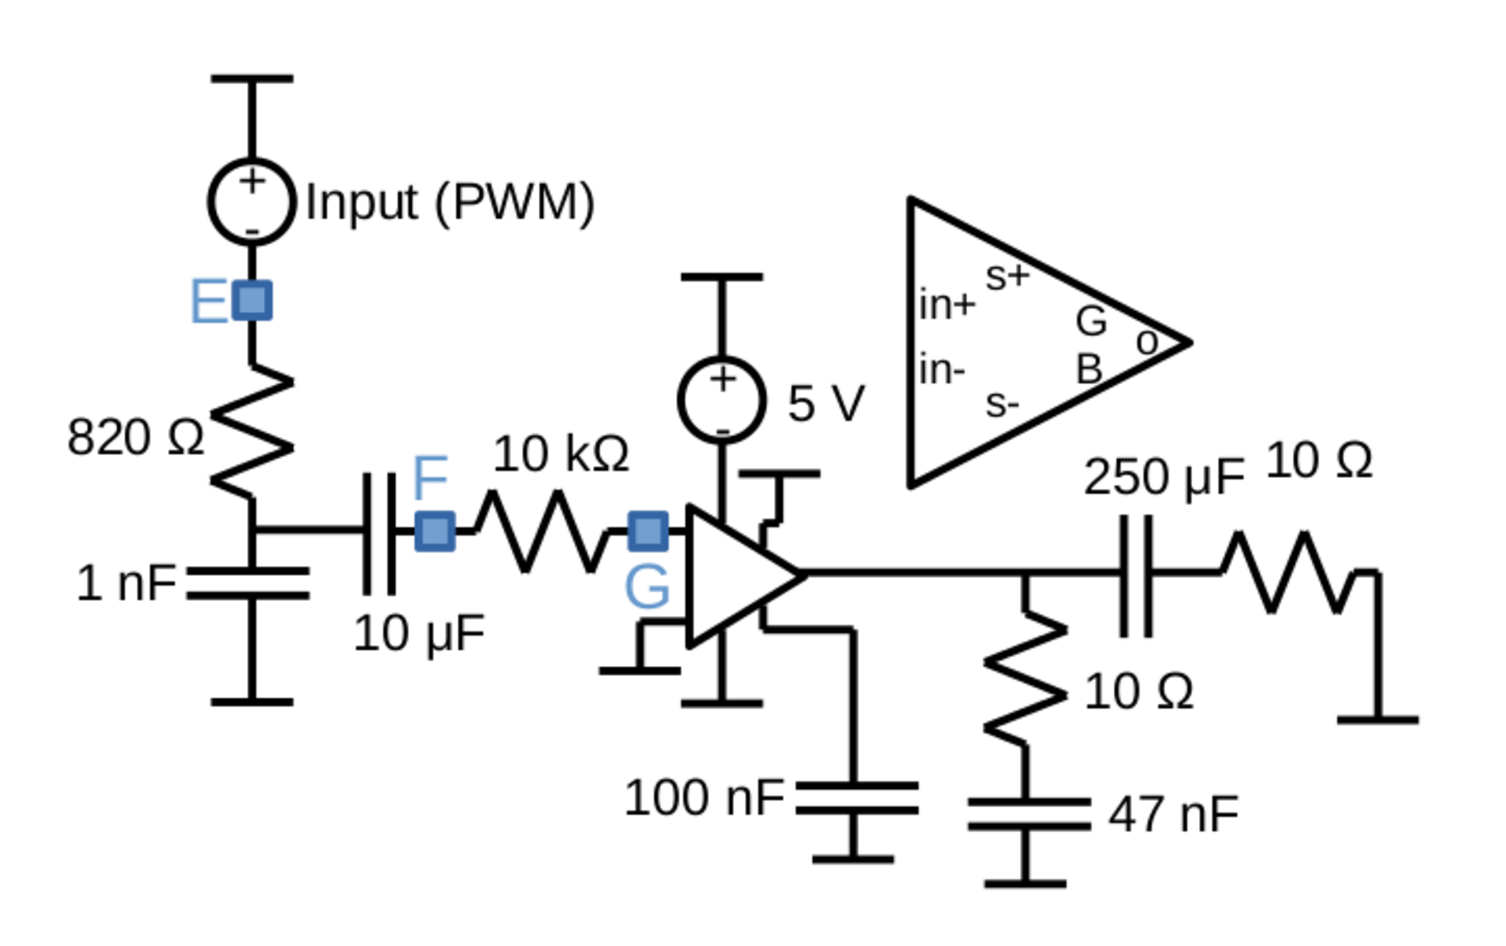
\includegraphics[scale=0.3]{AmpPar}	
		\end{figure}
		\column{0.4\textwidth}
		\begin{table}
			\centering
			\begin{tabular}{c|c}
				Punto & Tensión\\
				\hline \hline
				E & $(1.88;0.02)V$  \\
				\hline
				F & $(1.87;0.02)V$\\
				\hline
				G & $(0.000;0.002)V$\\
				\hline
				H & $(0.000;0.002)V$\\
				\hline
			\end{tabular}
		\end{table}
	\end{columns}
\end{frame}